\documentclass[11pt]{article}
\usepackage{geometry, graphicx, amssymb, amsmath, epstopdf}
\geometry{letterpaper}
\DeclareGraphicsRule{.tif}{png}{.png}{`convert #1 `dirname #1`/`basename #1 .tif`.png}
\newcounter{eoceSolCh}
\setcounter{eoceSolCh}{0}
\newcommand{\eoceSolCh}[1]{
\refstepcounter{eoceSolCh}\noindent\textbf{\arabic{eoceSolCh}\hspace{2mm}#1}

\addvspace{2mm}

}
\newcounter{eoceSol}[eoceSolCh]
\newcommand{\eoceSol}[1]{\refstepcounter{eoceSol}\noindent\small\textbf{\arabic{eoceSolCh}.\arabic{eoceSol}}\hspace{2mm}#1\addtocounter{eoceSol}{1}

\addvspace{1mm}

}
\begin{document}


%%%%%%%%%%%%%%%%%%%%%%%

\setcounter{eoceSolCh}{1}
\eoceSolCh{Probability}

\eoceSol{False. The tosses are independent trials.}

\eoceSol{(a) 10 tosses. With a low number of flips the variability in the number of heads observed is much larger, so a result further from 50\% is more likely. (b) 100 tosses. With more flips, the observed proportion of heads would probably be closer to 50\% and therefore above 40\%. (c) 100 tosses. The more flips, the less variability away from 50\%. (d) 10 tosses. Fewer flips mean more volatility and a greater chance of getting far from 50\% and below 30\%.}


\eoceSol{(a) $1/1024$. (b) $1/1024$. (c) $1023/1024$.}

\eoceSol{(a) Figure below. (b) 0.05 (c) 0.70 (d) 0.95 (e) 0.05 (f) No, there are bloggers who own both types of cameras.}
%\includegraphics[width=50mm]{02/figures/eoce/psDslrVenn.png}

\eoceSol{(a) Yes. (b) Yes. (c) No.)}

\eoceSol{(a) 0.26. (b) 0.23. (c) 0.0598. (d) We assumed that the education level of the husband and wife are independent. This may not be an unreasonable assumption since people often marry people who have a comparable level of education to theirs.}

\eoceSol{(a) Sum greater than 1. (b) This one is okay. (c) Sum less than 1. (d) Negative probabilities make no sense. (e) This one is okay. (f) Probabilities cannot be less than 0 or greater than 1.}

\eoceSol{(a) 0.4236. (b) 0.1458. (c) 0.1875. (d) 0.0625.}

\eoceSol{(a) The distribution is right skewed, with a median between 0 and 50,000. Values range from 0 to 500,000 and there are potential outliers on the higher end. (b) 0.8696. (c) 0.4808. (d) 0.4181. (e) Probably not. It appears that females on average make less money than men, i.e. independence does not hold.}

\eoceSol{No.}

\eoceSol{(a) 0.2825. (b) 0.4167. (c) 0.1905. (d) No, because P(black hair $|$ brown eyes) $\ne$ P(black hair $|$ blue eyes). (Other explanations are possible.)}

\eoceSol{(a) 0.65. (b) 0.72. (c) 0.468. (d) We assumed that the burger preferences of the man and the woman are independent. This may not be a reasonable assumption. (e) 0.514.}

\eoceSol{Female.}

\eoceSol{0.6049.}

\eoceSol{(a) Tree diagram below. (b) 0.68. (c) 0.32.}
%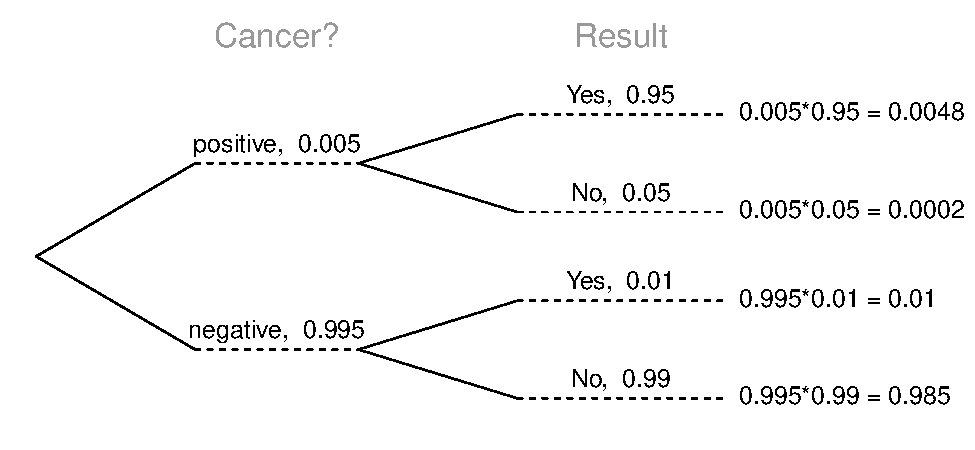
\includegraphics[width=60mm]{02/figures/eoce/cancerTree.pdf}

\eoceSol{(a) Tree diagram below. (b) 0.84.}
%\includegraphics[width=60mm]{02/figures/eoce/constructBoxPlot.pdf}

\eoceSol{(a) 0.3. (b) 0.3. (c) 0.3. (d) 0.09. (e) No, the draws are independent.}


\eoceSol{(a) 0.091. (b) 0.318. (c) 0.455. (d) 0. (e) 0.288.}

\eoceSol{0.0519.}

\eoceSol{(a) 13. (b) No, this would be unreliable. The students are not a random sample.}

\eoceSol{(a) Probability model below. Expected winnings: \$3.59. (b) EV: -\$1.41, SD: \$3.37. (c) No. The expected net profit is negative so on average you expect to lose money.}
{\scriptsize\begin{tabular}{llll}
\hline
Event	& 3 hearts & 3 blacks & Else \\
\hline
$X$		& \$50	& \$25	& \$0 \\
$P(X)$	& 0.0129	& 0.1176	& 0.8695 \\
\hline
\end{tabular}} \vspace{1mm}

\eoceSol{(a) EV: -\$0.16, SD: \$3. (b) EV: -\$0.16, SD: \$1.73. (c) Expected values are the same but the standard deviations are different. The standard deviation from the game where winnings and losses are tripled is higher, making this game riskier.}

\eoceSol{(a) Probability model below. Expected winnings: -\$0.54 (b) No, he is expected to lose money on average.}
{\scriptsize\begin{tabular}{lllll}
\hline
Event	& Number	& J, Q, K	& Ace	& A$\clubsuit$ \\
\hline
$X$		& -2		& 1		& 3		& 23 \\
$P(X)$	& 0.6923	& 0.2308	& 0.0577	& 0.0192 \\
\hline
\end{tabular}} \vspace{1mm}

\eoceSol{\$4.26.}

\eoceSol{(a) Mean: \$3.90, SD: \$0.34. (b) Mean: \$27.30, SD: \$0.89.}

























\end{document}  